
\section{Counterexample} \label{sec:counterexample}

\begin{figure}[t]
	\centering
	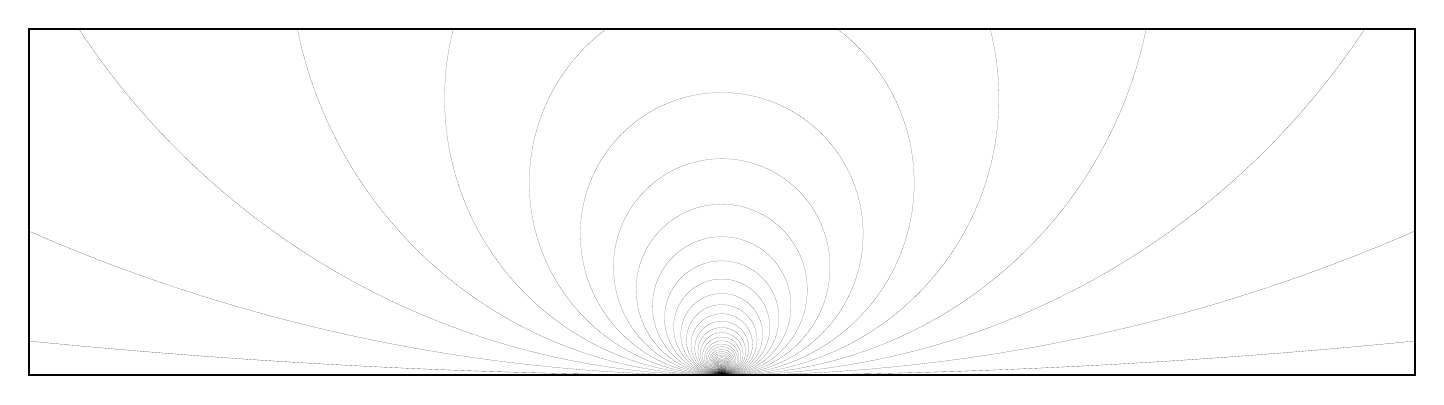
\begin{tikzpicture}[scale=88]
	\draw[thick] (-.1,0) rectangle (.1,.05);
	\clip (-.1,0) rectangle (.1,.05); % remove for all circles
	\foreach \i in {1,...,100}{
		\draw[line width=0.1/\i mm] (0, 1/\i^2) circle (1/\i^2);
	}
	\end{tikzpicture}
	\caption{A closeup of the Hawaiian hearing $\mathbb{H}^1$.}
	\label{fig:earrings}
\end{figure}

In this section we show that a sublevel filtration can be $\HLC$ and not q-tame for most homology theories of interest.

The \textit{$d$-dimensional Hawaiian earring}, see Figure \ref{fig:earrings}, is defined as the subspace
\begin{equation*}
\HE = \bigcup_{n\in\mathbb{N}}\left\{(x_0,\dots,x_d)\in\R^{d+1}\mid \left(x_0-\frac{1}{n}\right)^2+x_1^2+\dots+x_d^2=\left(\frac{1}{n}\right)^2\right\}
\end{equation*}
of $d+1$-dimensional Euclidean space.

\begin{thm} \label{thm:counterexample}
	Let $\H$ be a homology theory such that its value on a point is finitely generated for every degree and on $\HE$ is not finitely generated for some degree. Then, the function $f \colon \HE \to \R$ whose value at the origin is $0$ and is $1$ everywhere else defines a $\HLC$ Morse filtration that is not q-tame.
\end{thm}

\begin{proof}
	The space $\HE$ is Hausdorff and locally compact since $R^{d+1}$ is.
	To verify that $(\HE,f)$ is a Morse filtration we notice that all level sets are either the empty set, the singleton containing the origin, or $\HE$ itself, all compact spaces.
	Let us now verify that $\HE$ is $\HLC$.
	Let $\epsilon > 0$ and $x \in \HE$.
	If $x$ is the origin, we choose $\delta$ between $0$ and the minimum of $\epsilon$ and $1$.
	Then $\HE_{\leq f(x) + \delta} = \HE_{\leq \delta} = \{x\}$, so the desired condition follows from the first assumption on the homology theory.
	For $x$ not the origin, there is a unique $d$-sphere that contains it.
	Clearly, we may choose $\delta > 0$ so small that $D_\delta(x) = \{y \in \R^{d+1} \mid \Vert x - y \Vert < \delta\} \cap \HE$ is contained in this sphere, so $D_\delta(x)$ is homotopy equivalent to a $x$ and the condition again follows trivially.
	What remains to be shown is that $\HE_{\leq \bullet}$ is not q-tame.
	Since $\HE_{\leq t}$ is constant with value $\HE$ for $t \geq 1$, the second assumption on the homology theory finishes the proof.
\end{proof}

\begin{prop}
	The assumptions of Theorem~\ref{thm:counterexample} are satisfied by singular and \v{Cech} homology.
\end{prop}

\begin{proof}
	The case of singular homology is well know and can be found in \cite{Barratt.1962}.
	For \v{C}ech homology we use the fact that it commutes with inverse limits for compact Hausdorff spaces.
	Define 
	\begin{align*}
	\HE_k &= \left\{(x_0,\dots,x_d)\in\R^{d+1}\mid \left(x_0-\frac{1}{k}\right)^2+x_1^2+\dots+x_d^2=\left(\frac{1}{k}\right)^2\right\}\\
	&\cup\bigcup_{n=1}^{k-1}\left\{(x_0,\dots,x_d)\in\R^{d+1}\mid \left(x_0-\frac{1}{n}\right)^2+x_1^2+\dots+x_d^2=\left(\frac{1}{n}\right)^2\right\},
	\end{align*}
	i.e., the $d$-dimensional Hawaiian earring but with the $k$-th largest $d$-sphere filled.
	We have $\lim_{k}\HE_{k} = \bigcap_{k}\mathbb{H}^{d}_{k}=\mathbb{H}^{d}$, and hence $\CH_{d}(\HE) = \lim_{k}\CH_{d}(\mathbb{H}^{d}_{k})$.
	One can easily check that each $\mathbb{H}^{d}_{k}$ satisfies the assumptions for \cref{prop:cech_sing_hom_hlc}, which implies $\lim_{k}\CH_{d}(\mathbb{H}^{d}_{k})=\lim_{k}H_{d}(\mathbb{H}^{d}_{k})$.
	We compute
	\begin{equation*}
	\lim_{k}H_{d}(\mathbb{H}^{d}_{k})=\lim\left(\dots\to \prod_{n=1}^2\mathbb{F}\to \prod_{n=1}^1\mathbb{F}\to \prod_{n=1}^0\mathbb{F}\right)=\prod_{n\in\mathbb{N}}\mathbb{F},
	\end{equation*}
	which is infinite-dimensional over $\mathbb{F}$.
	This finishes the proof.
\end{proof}